\ifx\allfiles\undefined
\documentclass[12pt, a4paper, oneside, UTF8]{ctexbook}
\def\path{../config}
\usepackage{amsmath}
\usepackage{amsthm}
\usepackage{array}
\usepackage{amssymb}
\usepackage{graphicx}
\usepackage{mathrsfs}
\usepackage{enumitem}
\usepackage{geometry}
\usepackage[colorlinks, linkcolor=black]{hyperref}
\usepackage{stackengine}
\usepackage{yhmath}
\usepackage{extarrows}
% \usepackage{unicode-math}
\usepackage{esint}
\usepackage{multirow}
\usepackage{fancyhdr}
\usepackage[dvipsnames, svgnames]{xcolor}
\usepackage{listings}
\usepackage{float} % Required for the H float option
\definecolor{mygreen}{rgb}{0,0.6,0}
\definecolor{mygray}{rgb}{0.5,0.5,0.5}
\definecolor{mymauve}{rgb}{0.58,0,0.82}
\definecolor{NavyBlue}{RGB}{0,0,128}
\definecolor{Rhodamine}{RGB}{255,0,255}
\definecolor{PineGreen}{RGB}{0,128,0}

\graphicspath{ {figures/},{../figures/}, {config/}, {../config/} }

\linespread{1.6}

\geometry{
    top=25.4mm, 
    bottom=25.4mm, 
    left=20mm, 
    right=20mm, 
    headheight=2.17cm, 
    headsep=4mm, 
    footskip=12mm
}

\setenumerate[1]{itemsep=5pt,partopsep=0pt,parsep=\parskip,topsep=5pt}
\setitemize[1]{itemsep=5pt,partopsep=0pt,parsep=\parskip,topsep=5pt}
\setdescription{itemsep=5pt,partopsep=0pt,parsep=\parskip,topsep=5pt}

\lstset{
    language=Mathematica,
    basicstyle=\tt,
    breaklines=true,
    keywordstyle=\bfseries\color{NavyBlue}, 
    emphstyle=\bfseries\color{Rhodamine},
    commentstyle=\itshape\color{black!50!white}, 
    stringstyle=\bfseries\color{PineGreen!90!black},
    columns=flexible,
    numbers=left,
    numberstyle=\footnotesize,
    frame=tb,
    breakatwhitespace=false,
} 

\lstset{
    language=TeX, % 设置语言为 TeX
    basicstyle=\ttfamily, % 使用等宽字体
    breaklines=true, % 自动换行
    keywordstyle=\bfseries\color{NavyBlue}, % 关键字样式
    emphstyle=\bfseries\color{Rhodamine}, % 强调样式
    commentstyle=\itshape\color{black!50!white}, % 注释样式
    stringstyle=\bfseries\color{PineGreen!90!black}, % 字符串样式
    columns=flexible, % 列的灵活性
    numbers=left, % 行号在左侧
    numberstyle=\footnotesize, % 行号字体大小
    frame=tb, % 顶部和底部边框
    breakatwhitespace=false % 不在空白处断行
}

% \begin{lstlisting}[language=TeX] ... \end{lstlisting}

% 定理环境设置
\usepackage[strict]{changepage} 
\usepackage{framed}

\definecolor{greenshade}{rgb}{0.90,1,0.92}
\definecolor{redshade}{rgb}{1.00,0.88,0.88}
\definecolor{brownshade}{rgb}{0.99,0.95,0.9}
\definecolor{lilacshade}{rgb}{0.95,0.93,0.98}
\definecolor{orangeshade}{rgb}{1.00,0.88,0.82}
\definecolor{lightblueshade}{rgb}{0.8,0.92,1}
\definecolor{purple}{rgb}{0.81,0.85,1}

\theoremstyle{definition}
\newtheorem{myDefn}{\indent Definition}[section]
\newtheorem{myLemma}{\indent Lemma}[section]
\newtheorem{myThm}[myLemma]{\indent Theorem}
\newtheorem{myCorollary}[myLemma]{\indent Corollary}
\newtheorem{myCriterion}[myLemma]{\indent Criterion}
\newtheorem*{myRemark}{\indent Remark}
\newtheorem{myProposition}{\indent Proposition}[section]

\newenvironment{formal}[2][]{%
	\def\FrameCommand{%
		\hspace{1pt}%
		{\color{#1}\vrule width 2pt}%
		{\color{#2}\vrule width 4pt}%
		\colorbox{#2}%
	}%
	\MakeFramed{\advance\hsize-\width\FrameRestore}%
	\noindent\hspace{-4.55pt}%
	\begin{adjustwidth}{}{7pt}\vspace{2pt}\vspace{2pt}}{%
		\vspace{2pt}\end{adjustwidth}\endMakeFramed%
}

\newenvironment{definition}{\vspace{-\baselineskip * 2 / 3}%
	\begin{formal}[Green]{greenshade}\vspace{-\baselineskip * 4 / 5}\begin{myDefn}}
	{\end{myDefn}\end{formal}\vspace{-\baselineskip * 2 / 3}}

\newenvironment{theorem}{\vspace{-\baselineskip * 2 / 3}%
	\begin{formal}[LightSkyBlue]{lightblueshade}\vspace{-\baselineskip * 4 / 5}\begin{myThm}}%
	{\end{myThm}\end{formal}\vspace{-\baselineskip * 2 / 3}}

\newenvironment{lemma}{\vspace{-\baselineskip * 2 / 3}%
	\begin{formal}[Plum]{lilacshade}\vspace{-\baselineskip * 4 / 5}\begin{myLemma}}%
	{\end{myLemma}\end{formal}\vspace{-\baselineskip * 2 / 3}}

\newenvironment{corollary}{\vspace{-\baselineskip * 2 / 3}%
	\begin{formal}[BurlyWood]{brownshade}\vspace{-\baselineskip * 4 / 5}\begin{myCorollary}}%
	{\end{myCorollary}\end{formal}\vspace{-\baselineskip * 2 / 3}}

\newenvironment{criterion}{\vspace{-\baselineskip * 2 / 3}%
	\begin{formal}[DarkOrange]{orangeshade}\vspace{-\baselineskip * 4 / 5}\begin{myCriterion}}%
	{\end{myCriterion}\end{formal}\vspace{-\baselineskip * 2 / 3}}
	

\newenvironment{remark}{\vspace{-\baselineskip * 2 / 3}%
	\begin{formal}[LightCoral]{redshade}\vspace{-\baselineskip * 4 / 5}\begin{myRemark}}%
	{\end{myRemark}\end{formal}\vspace{-\baselineskip * 2 / 3}}

\newenvironment{proposition}{\vspace{-\baselineskip * 2 / 3}%
	\begin{formal}[RoyalPurple]{purple}\vspace{-\baselineskip * 4 / 5}\begin{myProposition}}%
	{\end{myProposition}\end{formal}\vspace{-\baselineskip * 2 / 3}}


\newtheorem{example}{\indent \color{SeaGreen}{Example}}[section]
\renewcommand{\proofname}{\indent\textbf{\textcolor{TealBlue}{Proof}}}
\newenvironment{solution}{\begin{proof}[\indent\textbf{\textcolor{TealBlue}{Solution}}]}{\end{proof}}

% 自定义命令的文件

\def\d{\mathrm{d}}
\def\R{\mathbb{R}}
%\newcommand{\bs}[1]{\boldsymbol{#1}}
%\newcommand{\ora}[1]{\overrightarrow{#1}}
\newcommand{\myspace}[1]{\par\vspace{#1\baselineskip}}
\newcommand{\xrowht}[2][0]{\addstackgap[.5\dimexpr#2\relax]{\vphantom{#1}}}
\newenvironment{mycases}[1][1]{\linespread{#1} \selectfont \begin{cases}}{\end{cases}}
\newenvironment{myvmatrix}[1][1]{\linespread{#1} \selectfont \begin{vmatrix}}{\end{vmatrix}}
\newcommand{\tabincell}[2]{\begin{tabular}{@{}#1@{}}#2\end{tabular}}
\newcommand{\pll}{\kern 0.56em/\kern -0.8em /\kern 0.56em}
\newcommand{\dive}[1][F]{\mathrm{div}\;\boldsymbol{#1}}
\newcommand{\rotn}[1][A]{\mathrm{rot}\;\boldsymbol{#1}}

% 修改参数改变封面样式,0 默认原始封面、内置其他1、2、3种封面样式
\def\myIndex{0}


\ifnum\myIndex>0
    \input{\path/cover_package_\myIndex}
\fi

\def\myTitle{标题:一份LaTeX笔记模板}
\def\myAuthor{作者名称}
\def\myDateCover{封面日期: \today}
\def\myDateForeword{前言页显示日期: \today}
\def\myForeword{前言标题}
\def\myForewordText{
    
    这是一个基于\LaTeX{}的模板,用于撰写学习笔记。

    模板旨在提供一个简单、易用的框架,以便你能够专注于内容,而不是排版细节,如不是专业者,不建议使用者在模板细节上花费太多时间,而是直接使用模板进行笔记撰写。遇到问题,再进行调整解决。
}
\def\mySubheading{副标题}


\begin{document}
\input{\path/cover_text_\myIndex.tex}

\newpage
\thispagestyle{empty}
\begin{center}
    \Huge\textbf{\myForeword}
\end{center}
\myForewordText
\begin{flushright}
    \begin{tabular}{c}
        \myDateForeword
    \end{tabular}
\end{flushright}

\newpage
\pagestyle{plain}
\setcounter{page}{1}
\pagenumbering{Roman}
\tableofcontents

\newpage
\pagenumbering{arabic}
\setcounter{chapter}{-1}
\setcounter{page}{1}

\pagestyle{fancy}
\fancyfoot[C]{\thepage}
\renewcommand{\headrulewidth}{0.4pt}
\renewcommand{\footrulewidth}{0pt}








\else
\fi

\chapter{水泥}

\section{成分组成}

\begin{itemize}
	\item 硅酸三钙(简称C3S)——其矿物组成为3CaO·SiO2,含量约50\%
	\item 硅酸二钙(简称C2S)——其矿物组成为2CaO·SiO2,含量约20\%
	\item 铝酸三钙(简称C3A)——其矿物组成为3CaO·Al2O3,含量7\%~15\%
	\item 铁铝酸四钙(简称C4AF)——其矿物组成为4CaO·Al2O3·Fe2O3,含量10\%~18\%
\end{itemize}
其它矿物组成——硅酸盐水泥熟料中还含有少量的游离氧化钙和游离氧化镁及少量的碱(氧化钠和氧化钾)。它们可能对水泥的质量及应用带来不利影响。

\begin{table}[ht]
	\centering
	\begin{tabular}{|c|c|c|c|c|}
		\hline
		\textbf{性能指标} & \textbf{C$_3$S} & \textbf{C$_2$S} & \textbf{C$_3$A} & \textbf{C$_4$AF} \\ \hline
		水化速率          & 快              & 慢              & 最快            & 快              \\ \hline
		28天水化热        & 多              & 少              & 最多            & 中              \\ \hline
		强度              & 早期高          & 后期高          & 高              & 低              \\ \hline
		耐化学侵蚀        & 中              & 良              & 差              & 优              \\ \hline
		干缩性            & 中              & 小              & 大              & 小              \\ \hline
	\end{tabular}
	\caption{水泥主要成分性能对比}
	\label{cement-composition} % 标签已正确定义
\end{table}

正如表~\ref{cement-composition}中所显示的,\textbf{$C_3A$}的凝结速度快,为了降低水化速度,掺入石膏,石膏和\textbf{$C_3A$}反应生成钙矾石,调节凝结时间。但是石膏掺量过多时,可能导致膨胀性问题,从而危害水泥石的安定性。

\begin{table}[htbp]
	\centering
	\begin{tabular}{|c|c|c|c|}
		\hline
		\textbf{产品} & \textbf{结构形态} & \textbf{含量} & \textbf{性能} \\ \hline
		水化硅酸钙 & 胶体 & 50\% & 几乎不溶于水,胶凝性好、强度高 \\ \hline
		水化铝酸钙 & 立方晶体 & 25\% & 溶于水,强度低 \\ \hline
		水化铁酸钙 & 胶体 & 25\% & 棱柱状,难溶于水,胶凝性差,强度低 \\ \hline
		水化硫酸铝钙 & 针状晶体(单硫型板状) & 25\% & 不溶于水,强度高,可提高水泥早期强度 \\ \hline
		氯化钙 & 板状、六方片状晶体 & 25\% & 溶于水,强度较高 \\ \hline
	\end{tabular}
	\caption{凝结产物}
\end{table}

\textbf{常见的活性混合材料(又叫活性骨料):}

\begin{enumerate}
	\item \textbf{石膏}:
	主要用于调节水泥的凝结时间,从而延缓水泥的凝结过程。
	
	\item \textbf{矿渣}:
	在水泥中可以与水反应生成水化硅酸盐,促进水泥的硬化。
	
	\item \textbf{粉煤灰}:
	与水泥中的钙化合物反应,形成水化硅酸盐,增强水泥的后期强度和耐久性。粉煤灰的掺入有助于降低水泥的热释放,减少裂缝的产生,并提高其抗渗性和抗冻性。
\end{enumerate}

掺入活性混合材料的水泥的水化速度较慢,故早期强度较低,而由于水泥中熟料含量相对减少,故水化热较低、抗侵蚀性提高。

\begin{table}[ht]
	\centering
	\begin{tabular}{|c|p{10cm}|}
		\hline
		\textbf{水化阶段} & \textbf{特点与描述} \\ \hline
		\textbf{1) 水化早期} & 水化反应速度快; 水化产物形成速度大于扩散速度,溶液达到局部饱和; 1h左右,水泥颗粒表面被凝胶状膜层覆盖,水化反应速度下降。 \\ \hline
		\textbf{2) 水化中期} & 膜层不断增厚; 因内部水泥反应和凝胶吸水,凝胶膜破裂,水泥颗粒重新暴露,加速水化; 因水的蒸发,胶粒增大,相互吸引而凝聚,浆体成糊状。 \\ \hline
		\textbf{3) 水化后期} & 水化产物结晶,起到骨架作用,胶体填充晶体之间的空隙,水泥石密实度增加,成为具有一定强度的整体。 \\ \hline
	\end{tabular}
	\caption{水泥水化过程各阶段特点}
\end{table}

\begin{remark}
水泥凝结硬化速度的影响因素:

1.水泥的熟料矿物组成

水泥熟料中各种矿物的凝结硬化特点不同,C3S、C3A含量高,水泥凝结硬化速度快,C2S含量高,水泥凝结硬化速度慢。

2.水泥的粉磨细度

水泥磨得愈细,水泥颗粒平均粒径小,比表面积大,水化时与水的接触面大,水化速度快,凝结硬化快,早期强度就高。

3. 水泥浆的水灰比

水泥浆的水灰比是指水泥浆中水与水泥的质量之比。当水泥浆中加水较多时,水灰比较大,此时水泥的初期水化反应得以充分进行;但是水泥颗粒间原来被水隔开的距离较远,颗粒间相互连接形成骨架结构所需的凝结时间长,所以水泥浆凝结较慢,且空隙多,降低水泥石的强度。
\end{remark}

\section{水泥技术性质、侵蚀、材料选择}\label{feature}
水泥特性与应用:(1)\textbf{凝结硬化快},早强和后强均较高(2)\textbf{抗冻性好}(3)\textbf{水化热高}(不适用于大体积混凝土工程)(4)\textbf{耐腐蚀性、耐热性差}

水泥的技术性质从这几个方面进行评价:
\begin{enumerate}
	\item \textbf{细度:}
	指水泥颗粒的粗细程度。
	\item \textbf{凝结时间:}
	分为初凝和终凝,初凝最好慢一点方便水泥塑形等操作,终凝最好快一点方便施工。
	\item \textbf{体积安定性:}
	水泥安定性不良的原因是由于其熟料矿物组成中含有过多的游离氧化钙或游离氧化镁,以及水泥粉磨时所掺石膏超量等所致。熟料中所含的游离氧化钙或游离氧化镁都是在高温下生成的,属过烧石灰,水化很慢,它要在水泥凝结硬化后才慢慢开始水化,水化时产生体积膨胀,从而引起不均匀的体积变化而使硬化水泥石开裂。
	\item \textbf{强度:}
	分为普通型和早强型,有代号R者为早强型,比如62.5R
	\item \textbf{碱含量}
\end{enumerate}

掺入活性骨料的水泥:掺入活性混合材料的水泥的水化速度较慢,故早期强度较低,而由于水泥中熟料含量相对减少,故水化热较低、抗侵蚀性提高。

简记表:

\begin{table}[ht]
	\centering
	\resizebox{\textwidth}{!}{ % 修复超宽表格
		\begin{tabular}{|c|c|c|c|c|c|c|}
			\hline
			\textbf{名称} & \textbf{硅酸盐水泥} & \textbf{普通水泥} & \textbf{矿渣水泥} & \textbf{火山灰水泥} & \textbf{粉煤灰水泥} & \textbf{复合水泥} \\
			\hline
			\textbf{成分} & 水泥熟料+石膏 & 掺少量活性材料 & 矿渣 & 火山灰 & 粉煤灰 & 多种复合添加 \\
			\hline
			\textbf{主要特征} & 同~\ref{feature} & 同~\ref{feature} & 和硅酸盐相反 & 和矿渣的区别是耐热较差 & 干缩性较小 & 早强高,其余提升 \\
			\hline
		\end{tabular}
	}
	\caption{含活性骨料的水泥} \label{table:cement}
\end{table}

\textbf{Trick:}

耐冻性和耐腐蚀性处处相反

\textbf{水泥的腐蚀:}

软水, 即含离子较少的水,如雨水、雪水、大部分河水、湖水。

腐蚀原因:$Ca(OH)_2$ 微溶于水

\begin{itemize}
	\item 对于静水或无压水,软水腐蚀仅限于表面
	\item 对于流动水或有压水,则会不断溶解,造成严重的损害
\end{itemize}

反应式: 
\[
Ca(OH)_2 + Ca(HCO_3)_2 \rightarrow 2CaCO_3 + 2H_2O
\]

\textbf{盐类腐蚀:}

\textbf{(1)硫酸盐腐蚀}:
\[
C_4AH_{13} + 3CS + 20H^- \rightarrow C_3A \cdot 3CS \cdot H_3SO_4 + CH
\]

\textbf{(2)铁盐腐蚀}:
\[
Mg^{2+} + Ca(OH)_2 \rightarrow Mg(OH)_2 + Ca^{2+}
\]

\textbf{酸类腐蚀:}

\textbf{(1)碳酸腐蚀}:
\[
Ca(OH)_2 + CO_2 + H_2O \rightarrow 2CaCO_3 + 2H_2O
\]
\[
CaCO_3 + H_2O + CO_2 \rightarrow Ca(HCO_3)_2
\]

\textbf{(2)一般酸腐蚀}:
与Ca(OH)₂反应生成酸碱中和反应生成盐

\textbf{强碱腐蚀}

\[
C_3A + 6NaOH \rightarrow N_3A + 3Ca(OH)_2
\]

在空气中干燥后,与空气中的CO₂反应生成Na₂CO₃,结晶吸水长大,引起膨胀。

从产物上看,主要有以下三种腐蚀类型:
\begin{enumerate}
	\item 生成可溶性产物
	\item 生成无胶凝能力产物
	\item 生成体积膨胀产物
\end{enumerate}

\newpage
完整表:

\begin{figure}[htbp]
	\centering
	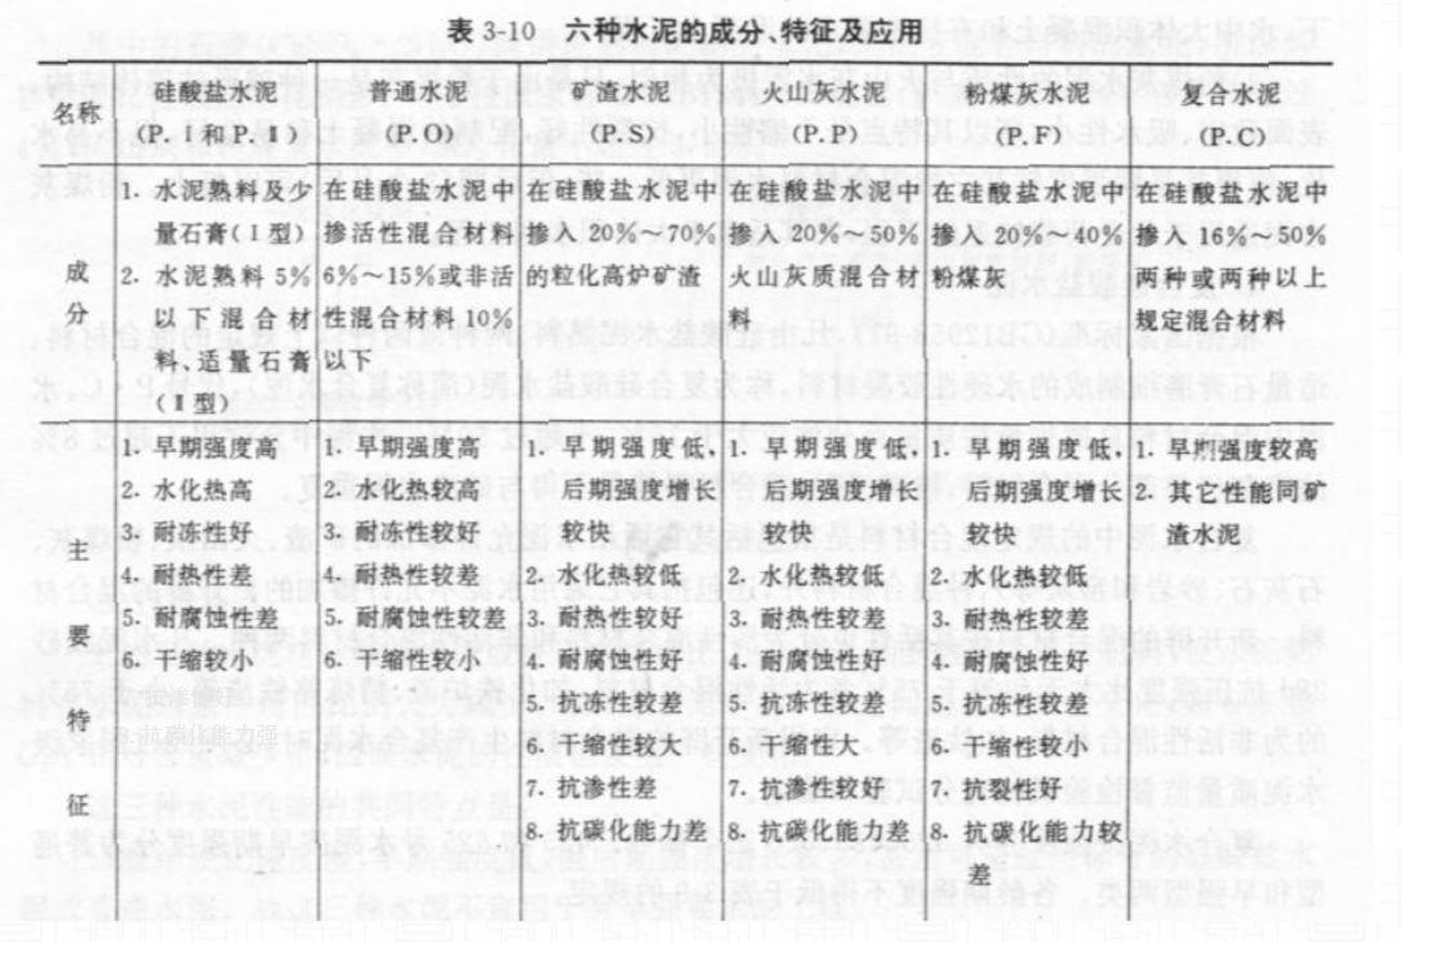
\includegraphics[width=0.7\linewidth]{../figure/sn1.png} % 确保图片路径正确
	\caption{}
	\label{fig:sn1}
\end{figure}

\begin{figure}[H]
	\centering
	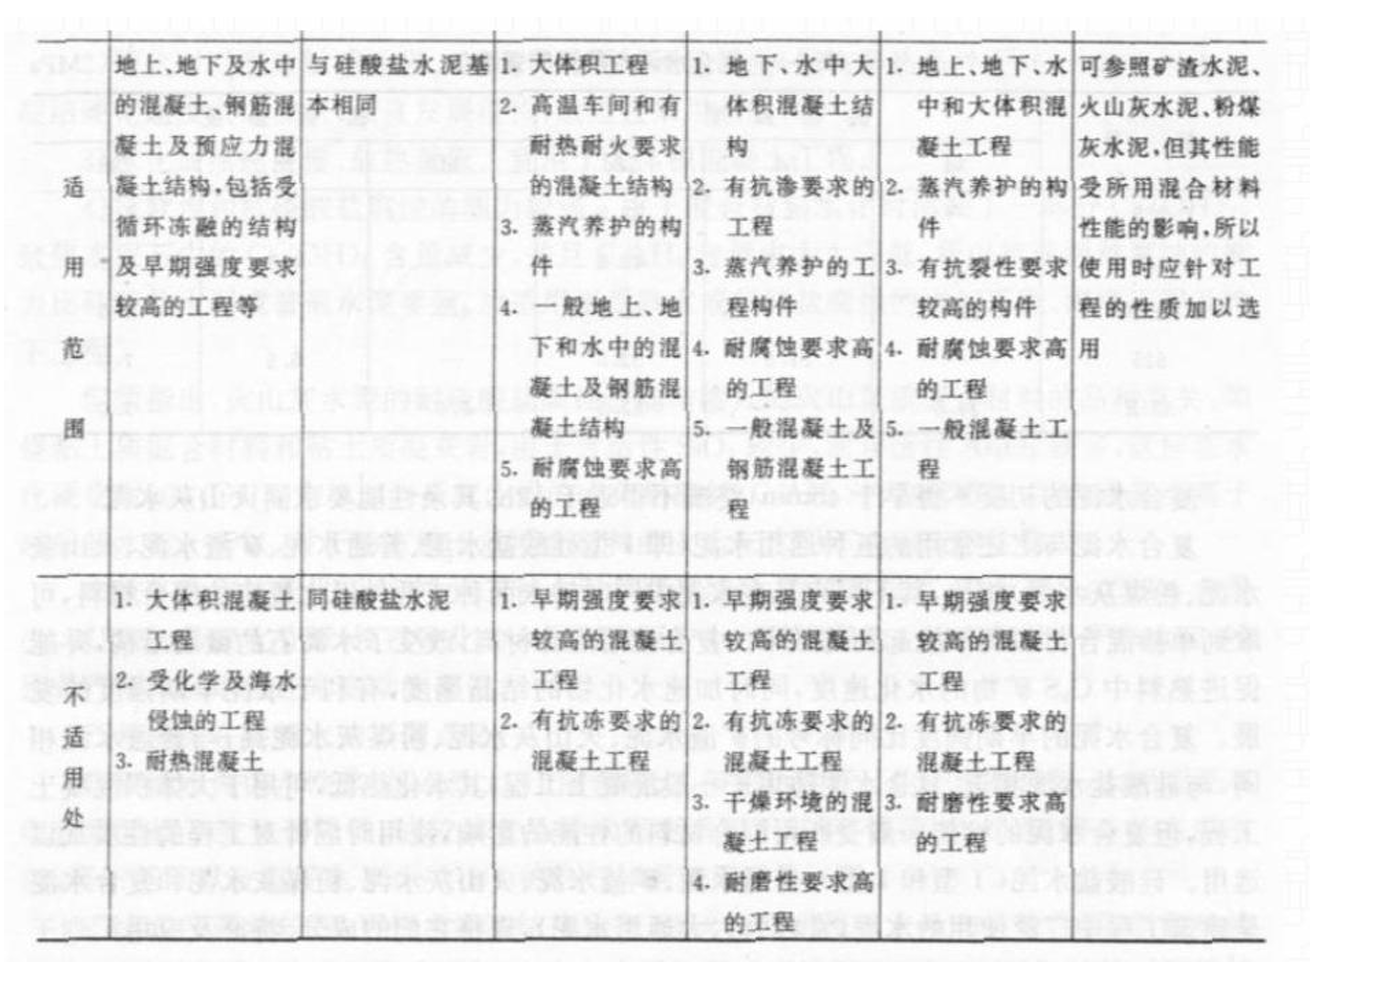
\includegraphics[width=0.7\linewidth]{../figure/sn2.png} % 确保图片路径正确
	\caption{}
	\label{fig:sn2}
\end{figure}

\newpage

\section{其他品种水泥}

\begin{enumerate}
	\item \textbf{快硬水泥}:参考~\ref{cement-composition},多加铝酸三钙,提高凝结速度
	\item \textbf{快凝快硬硅酸盐水泥:}掺杂硬石膏、矿渣,关键是磨细
	\item \textbf{抗硫酸盐水泥:}以硅酸钙为主的熟料,加入适量石膏,磨细生成的一种具有抗硫酸盐性能的水硬性胶凝材料
	\item \textbf{高铝水泥:}快凝早强,水化热大,抗硫酸盐性能很强,耐热性好,长期强度要降低
	\item \textbf{中低热水泥:}降低C3S和C3A的含量。
\end{enumerate}

\begin{remark}
掺杂大量混合材料的硅酸盐水泥的特性:

1. 凝结硬化建度慢,{\color{red}早期强度低。但后期强度增长较多。}甚至可超过同标号的硅酸盐水泥或普通水泥。故这三种水泥不宜用于有早强要求的工程。

2. {\color{red}硬化时对湿热敏感性强。温度低时凝结硬化缓慢},但在湿热条件下(60-70°C以上),凝结硬化速度大大加快,强度发展很快,故适宜采用蒸汽养护。

3. {\color{red}水化放热速度慢,放热量低}。宜用于大体积混凝土工程。

4. {\color{red}抗软水和抗硫酸盐腐蚀的能力较强}。

5. {\color{red}抗冻性和抗碳化能力差}。这三种水泥早期强度低。受冻易损害,且由于Ca(OH)₂含量少,碱度低,易碳化分解。使已硬化的水泥石表面产生“起粉”现象。故不宜用于严寒地区,特别是严寒地区水位经常变动的部位。
\end{remark}

\section*{作业题}

\begin{example}
	硅酸盐水泥熟料的主要矿物组成是什么?它们单独与水作用时的特性如何? 

	硅酸三钙C3S、硅酸二钙C2S、铝酸三钙C3A、铁铝酸四钙C4AF

	\begin{itemize}
		\item C3S:水化速率快,28天水化热多,早期强度高,耐化学侵蚀性中等,干缩性中等
		\item C2S:水化速率慢,28天水化热少,后期强度高,耐化学侵蚀性良好,干缩性小
		\item C3A:水化速率最快,28天水化热最多,强度高,耐化学侵蚀性差,干缩性大
		\item C4AF:水化速率快,28天水化热中等,强度低,耐化学侵蚀性优良,干缩性小
	\end{itemize}
	\textbf{注意:水化速率快的矿物,28天水化热多,强度高,耐化学侵蚀性差,干缩性大}
	\textbf{水化速率慢的矿物,28天水化热少,强度低,耐化学侵蚀性良好,干缩性小}
\end{example}

\begin{example}
	硅酸盐水泥的主要水化产物是什么?硬化水泥石的结构怎样? 

	\begin{itemize}
		\item 硅酸盐水泥的主要水化产物是水化硅酸钙、氢氧化钙、氢氧化铝、氢氧化铁等。
		\item 硬化水泥石的结构是由水化硅酸钙和氢氧化钙等组成的胶体和晶体相互交织而成的多孔结构。
	\end{itemize}
	\textbf{注意:水化硅酸钙是主要的胶凝材料,氢氧化钙是水泥石的主要成分之一}
\end{example}

\begin{figure}[H]
	\centering
	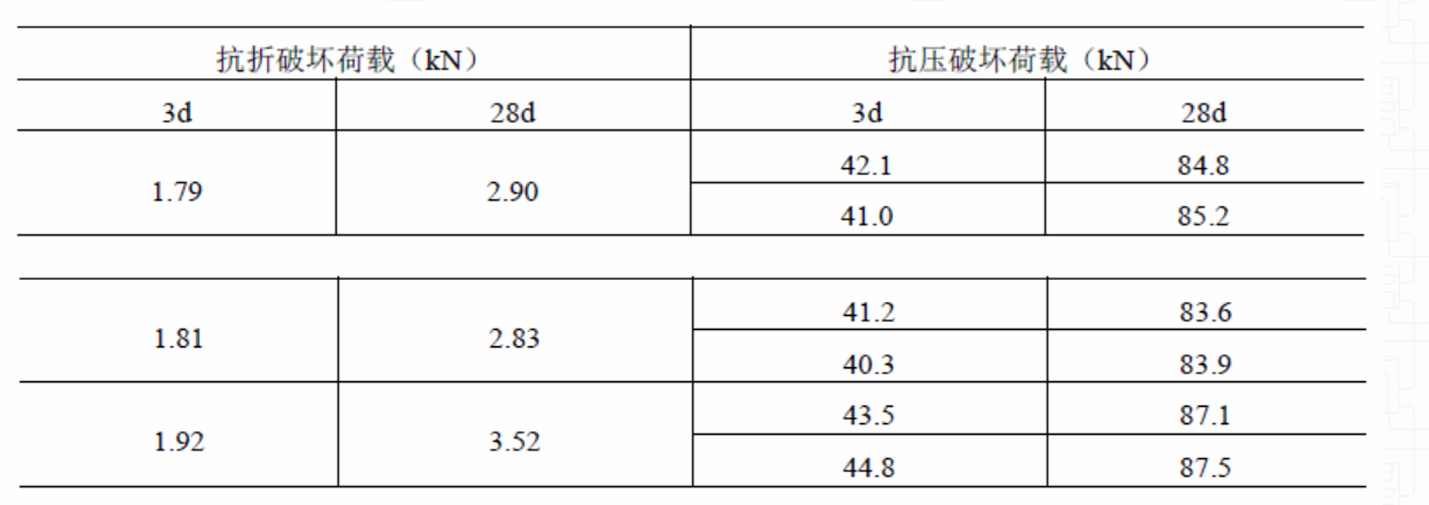
\includegraphics[width=0.7\linewidth]{../figure/qiangdudengji.png} % Ensure the file exists at this path
	\caption{水泥强度等级评定}
	\label{fig:qiangdudengji}
\end{figure}

\begin{example}
	为什么硅酸盐水泥里必须加入一定量石膏,添加石膏过多或过少会导致什么后果?

	制造通用硅酸盐水泥时掺入适量石膏主要是为了调节水泥的凝结时间。

硅酸盐水泥的四种熟料矿物中,C3A 的水化和凝结硬化速度最快,在无石膏存在时,它能使水泥瞬间产生凝结。C3A 的水化和凝结硬化速度可通过掺加适量石膏加以控制。在有石膏存在时,C3A 水化后易与石膏反应而生成难溶于水的钙矾石,它沉淀在水泥颗粒表面形成保护膜,阻碍 C3A 的水化,从而起到延缓水泥凝结的作用。

添加过少会导致凝结过快,无法保证混凝土和易性,添加过多会导致钙矾石生成过量,发生体积膨胀。同时也会导致混凝土安定性不良。

\end{example}

\begin{example}
	水泥胶砂的标准尺寸是什么?
	$$40mm \times 40mm \times 160mm$$
\end{example}

\begin{example}
	活性混合材料中含有()和()成分,他们能和水泥水化产生的Ca(OH)2作用,这一反应称为()。

	分别是活性二氧化硅($SiO_2$)和活性三氧化二铝($Al_2O_3$)。它们可以和氢氧化钙反应生成水化硅酸钙和水化铝酸钙。当有石膏,水化铝酸钙可以进一步反应生成水化硫铝酸钙。称石膏和氢氧化钙为活性材料的激发剂。

当然首先发生的还是水泥熟料的反应,其次是以上反应,被称为二次水化。

特点是:

\begin{itemize}
	\item 反应慢
	\item 消耗氢氧化钙,提高酸性环境下耐久性,减少碱骨料反应的膨胀
	\item 产生的水化产物是水硬性的,可以提高材料强度,填补孔隙
\end{itemize}
\end{example}

\begin{example}
	影响水泥水化和硬化的因素是什么?

	\begin{itemize}
		\item 组成成分(如上文所述)
		\item 细度(越细,比表面积越大,凝结越快,早期强度越高)
		\item 石膏掺量
		\item 水灰比(水灰比越大,强度越小)
		\item 养护条件(适宜的温度和较高的湿度有利于水化和硬化)
		\item 养护龄期
		\item 外加剂的使用
		\item 贮存条件
	\end{itemize}
	\end{example}

\ifx\allfiles\undefined
\end{document}
\fi